%--------------------------------------------------------------------------------------------------
% 
\chapter{Computational Framing Analysis}
\label{ch:nfa}
%--------------------------------------------------------------------------------------------------
Framing is a selection of particular aspects of factual events and rendering them salient to promote a particular interpretation, evaluation, and/or solution~\parencite{entman_framing_1993, entman_cascading_2003}.
Alternatively, a frame was presented as ``a central organizing principle that holds together and gives coherence and meaning to a diverse array of symbols''~\parencite{gamson1992media}.

Computational Framing Analysis (CFA) is a research field of communication framing detection and analysis using computation.
Since news texts are the most common type of communication used in the research community for CFA, we will be presenting its application in this context. 
Although framing is casually defined, computational framing analysis has been studied diversely~\parencite{ali-hassan-2022-survey}.

\section{Framing Theory and Its Relevance to News Analysis}

The same facts in news articles can be presented in various ways.
Media plays a crucial role in our society; therefore, observing and studying news framing is crucial to understanding its influences.
Framing can have many social consequences since it can shape public discourse and induce strong emotions towards specific topics that could otherwise be overlooked or marginalized.
It can promote specific perspectives influencing the public's perception, leading to different interpretations through carefully selected narratives.
It is often hidden in news articles and presented as content for casual reading.
News Framing can reflect dominant group influences by repeating and reinforcing specific views and topics.
Therefore Computational Framing Analysis is very important for today's overall understanding of ever-growing news content.
Computational Framing Analysis assists individuals in comprehending the reasons behind the dominance of particular viewpoints, while other equally significant perspectives have not gained prominence.

\section{Traditional Approaches to CFA}

CFA can be considered a Topic Modelling problem in an unsupervised setting or a multi-label classification problem when the supervised methods are applied.
Topic modelling is a type of statistical modelling used in Natural Language Processing (NLP) and machine learning for discovering abstract ``topics'' that occur in a collection of documents.
A topic in this context refers to a set of words that are frequently seen together in a document and capture a specific theme or subject.
When supervised methods in CFA are used, the text is usually annotated with multiple predetermined labels on various levels: whole article, title, body, paragraphs, or text spans.

\subsection{Unsupervised and Semi-supervised Approaches to CFA}
Traditionally CFA utilized various unsupervised methods. 
Unsupervised methods do not require labelled data but aim to discover hidden patterns or structures in the text. 
Some common unsupervised techniques for framing analysis include Topic Modelling (TM) with Latent Dirichlet Allocation (LDA) algorithm~\parencite{blei2003latent}. 
These algorithms aim to discover underlying topics or themes in large collections of documents and can be employed to reveal latent frames in the text~\parencite{blei2012probabilistic}.
The basic idea is that documents are represented as random mixtures over latent topics, where the topic is a probability distribution over a fixed vocabulary.
\textcite{dimaggio2013exploiting} employed LDA topic modelling to investigate the framing of government support for artists and arts organizations, with each topic being regarded as a distinct frame. 
Structural topic modelling (STM) was later applied in a similar fashion by~\textcite{roberts2014structural, gilardi2020policy}, which included not only topics from the text but also covariates present in document metadata (e.g. gender, origin, political affiliation, time trends etc...). 
%Focusing on smoking restriction in U.S. states, our analysis draws upon an original dataset of over 52,000 paragraphs from newspapers covering 49 states between 1996 and 2013
The STM was further improved by \textcite{nguyen-etal-2015-tea}, who introduced the supervised Hierarchical Topic Model - Supervised Hierarchical Latent Dirichlet Allocation (SHLDA). 
SHLDA can discover a hierarchy of topics from a collection of documents, each associated with the ideological (liberal, conservative) score of the text author (Member of the U.S. Congress).
In the learned hierarchy, first-level nodes map to the general topic (agenda, issue), while second-level nodes represent ideologically polarized frames of the corresponding issue.
\textcite{walter2019news} proposed ``Analysis of Topic Model Networks'' where they applied LDA topic modelling and then created a semantic network. 
In this network, topics represent nodes; their similarity relationships serve as edges.
Lastly, a community detection algorithm was employed to group the topics into distinct communities within the network based on the prevalence of these topics in similar documents.
%congresional debates corpus

K-means clustering with TF-IDF vector model was applied by \textcite{burscher2016frames} to CFA using also mean word sentiment from SentiWord to detect a positive or negative tone for a given frame. 
The ``elbow'' method was used to predetermine the number of frames - clusters.
In contrast to topic modelling, k-means clustering follows a single-membership approach, assigning each document to just one cluster.

\subsection{Supervised Approaches to CFA}
\textcite{boydstun2013identifying, boydstun2014tracking} developed a manually annotated corpus on which they used logistic regression binary text classifiers.
\textcite{card-etal-2016-analyzing} used logistic regression classifier with unsupervised Dirichlet Persona Model~\parencite{bamman-etal-2013-learning} (DPM). 
The logistic regression classifier with DPM achieved improved performance when utilizing a wide range of NLP features (e.g. unigrams, bigrams, parts of speech, named entities, dependency tuples, ...) compared to the simple bag-of-words approach. 

From this point forward, neural network models have been CFA's dominant supervised learning approaches.
\textcite{naderi-hirst-2017-classifying} out-performed LDA and TF-IDF approaches on sentence-level classification tasks by employing bidirectional LSTM~\parencite{hochreiter1997lstm, graves2013bilstm} (Bi-LSTM) and gated recurrent units~\parencite{cho-etal-2014-properties} (GRU).
\textcite{ji-smith-2017-neural} out-performed logistic regression classifier~\parencite{card-etal-2016-analyzing} using Bi-LSTM with discourse dependency tree embedding, where the attention mechanism was used for composing child nodes representation.
Both Bi-LSTM methods attained optimal results when using pre-trained GloVe~\parencite{pennington-etal-2014-glove} as the source for input word embeddings.

\textcite{liu-etal-2019-detecting} was one of the first in testing transformer-based Large Pre-trained Models (LPMs), showing that BERT~\parencite{devlin2018bert} surpassed Bi-LSTM and GRU models equipped with attention mechanisms.
\textcite{khanehzar-etal-2019-modeling} demonstrated that LPMs also significantly out-perform support vector machines (SVM) in all cross-context (across different corpora) and cross-subject (immigration and same-sex marriage) CFA tasks. 
It was again evident that RoBERTa~\parencite{liu2019roberta} out-performs BERT in framing classification tasks and can be further improved with Multi-task learning where parameters are shared for the first eleven transformer layers~\parencite{huguet-cabot-etal-2020-pragmatics}.
\textcite{mendelsohn-etal-2021-modeling} demonstrated simultaneous classification for multiple framing typologies using RoBERTa on custom social media corpus.
Apart from \textcite{field-etal-2018-framing}, which used a clustering lexicon construction approach with an automatic translation to the Russian language, multilingual CFA wasn't widely studied.

\section{Recent Research of Multilingual CFA}
Multilingual CFA recently gained traction with SemEval-2023 task 3, where sub-task two specifically targeted news framing in multiple languages~\parencite{piskorski-etal-2023-semeval-task3}. 
The provided corpora for the task contained only a few hundred samples for English, French, German, Italian, Polish, and Russian languages. 
At the same time, no samples were available for Spanish, Greek, and Georgian.
So the task was not only multilingual but also a zero- and a few-shoot supervised learning task.

The winning solution~\parencite{liao2023marseclipse} for four languages, French, German, Italian, and Polish, used the XLM-RoBERTa-Large transformer model as an encoder and implemented a multilingual and multi-label contrastive model on top of it.
Their system came second in the remaining two languages with training data (English and Russian).
Contrastive learning has been a widespread technique in computer vision for a long time. 
The process involves selecting a random example as an anchor, followed by choosing positive and negative examples in relation to the anchor. 
Subsequently, positive examples are drawn closer to the anchor, while negative examples are pushed further away.
They calculated combined loss from binary cross entropy loss and contrastive loss obtained using a supervised architecture~\parencite{khosla2021supervised} adapted to a multi-label problem.
Following the work on SimCSE model~\parencite{gao2022simcse}, they produced two independent views of the data obtained from the encoder using a dropout and then used one sample for contrastive loss and the other for binary cross entropy loss calculation.

One of the solutions~\parencite{reiterhaas2023mcpt} that won a challenge on an ``unseen'' Spanish language also used contrastive learning with a transformer model.
\textcite{reiterhaas2023mcpt} used a two-phase multi-stage training procedure which fine-tunes sentence embeddings in a contrastive manner inspired by SETFIT~\parencite{tunstall2022efficient}. 
The model is built on top of sentence transformers~\parencite{reimers-2019-sentence-bert} encoder where they used a contrastive loss function modelled after the HeroCon-Loss~\parencite{zheng-etal-2022-contrastive}.
%The initial phase, contrastive fine-tuning, is based on the concept that the embeddings of samples with similar labels should be close. In contrast, the embeddings of models with different label vectors should be distant.
The initial phase is comprised of head pre-training and contrastive fine-tuning stages. 
The result of the two-stage first phase can be used for zero-shot prediction. 
Extended first phase with post-training and later weight reinitialization for additional second phase fine-tuning was used for a few-shot-based prediction.

\section{Datasets and Resources}

\textcite{boydstun2013identifying, boydstun2014tracking} introduced a codebook referred to as the ``Policy Frames Codebook'' (PFC) and developed a manually annotated corpus.
The codebook was developed through brainstorming and iterative application to randomly selected texts based on the framing definition of \textcite{entman_framing_1993}.
\begin{table}[htb]
    \caption{List of frame dimensions defined by \textcite{boydstun2013identifying, boydstun2014tracking} and used in MFC corpus.}
	\label{tab:frames}
	\centering
    \resizebox{\textwidth}{!}{%
		\begin{tabular}{l}
            \hline
            \textbf{Economic}: costs, benefits, or other financial implications\\
            \textbf{Capacity and resources}: availability of physical, human or financial resources, and capacity of current systems\\
            \textbf{Morality}: religious or ethical implications\\
            \textbf{Fairness and equality}: balance or distribution of rights, responsibilities, and resources\\
            \textbf{Legality, constitutionality and jurisprudence}: rights, freedoms, and authority of individuals, corporations,\\
            and the government\\
            \textbf{Policy prescription and evaluation}: discussion of specific policies aimed at addressing problems\\
            \textbf{Crime and punishment}: effectiveness and implications of laws and their enforcement\\
            \textbf{Security and defence}: threats to the welfare of the individual, community, or nation\\
            \textbf{Health and safety}: health care, sanitation, public safety\\
            \textbf{Quality of life}: threats and opportunities for the individual's wealth, happiness, and well-being\\
            \textbf{Cultural identity}: traditions, customs, or values of a social group in relation to a policy issue\\
            \textbf{Public opinion}: attitudes and opinions of the general public, including polling and demographics\\
            \textbf{Political}: considerations related to politics and politicians, including lobbying, elections, \\
            and attempts to sway voters\\
            \textbf{External regulation and reputation}: international reputation or foreign policy of the U.S.\\
            \textbf{Other}: any coherent group of frames not covered by the above categories\\
            \hline
		\end{tabular}
  }
\end{table}
Through this process, they established 15 framing dimensions shown in Table~\ref{tab:frames}.

Utilizing the PFC, \textcite{card-etal-2015-media} provided a manually-annotated dataset of news reports called the ``Media Frames Corpus'' (MFC).
MFC is the most commonly used dataset for supervised CFA approaches. It comprises 13 national U.S. newspaper articles from 1990 to 2012, covering three policy issues: immigration, smoking, and same-sex marriage. 
Multiple coders annotated each headline, article lead, article body text spans and overall framing of an article.

Another annotated dataset, the ``Gun Violence Frame Corpus''~\parencite{liu-etal-2019-detecting}, was utilized in neural network-based models explored earlier and is also based on the framing definition of \textcite{entman_framing_1993}. 
In this dataset, the authors manually annotated 1,300 news headlines gathered from 21 U.S. media outlets. 
Employing nine pre-defined codes derived from the literature, multiple coders annotated each headline.

\textcite{IEGQ1B_2020} provides automatically and manually annotated news article corpus in seven languages. 
This corpus contained five framing dimensions (Economy, Labour market, Welfare, Security, and Culture) regarding migration issues and was also the basis for the Slovene language corpus we started to develop. 
The corpus includes annotations for both the framing of the title and the overall framing of the article.

\begin{figure}[htb]
	\centering
    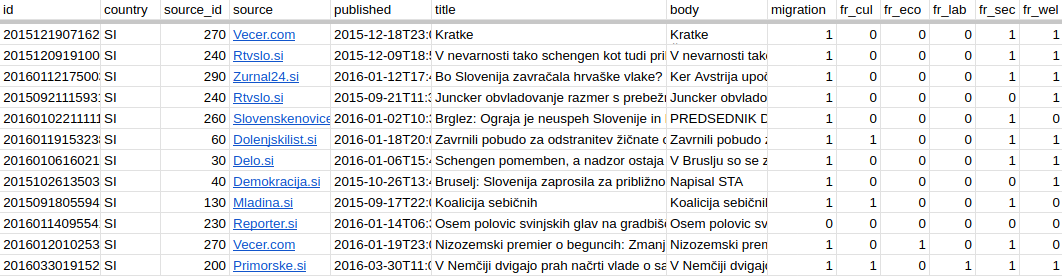
\includegraphics[width=1\textwidth]{figures/nf_corpora-1.png}
	\caption{REMINDER project framing corpus~\parencite{IEGQ1B_2020} structure example in the Slovene language with five framing labels (Culture, Economy, Labour market, Security, and Welfare) in the right-most columns and each article in a row.}
	\label{fig:nf_corpora}
\end{figure}

\section{Our Preliminary Research}

Our task was to compare Slovenian news frames of two European migration crises caused by the war in Syria and Ukraine. 
We used an automatically annotated news corpus~\parencite{IEGQ1B_2020} developed for the REMINDER project to train the multilingual frame classifiers.
Corpus consisted of migration news articles in seven languages and was annotated with five universal frames regarding migration.
We aimed to test Zero-shot Framing detection for the Slovene language not included in the corpus. 
Therefore, we have chosen two multilingual pre-trained transformer models XLM-RoBERTa and BERT and fine-tuned them on the migration corpus for multi-label classification. 
Furthermore, we used two classical transformation methods to tackle multi-label classification problems: Binary Relevance and Label Power-set ~\parencite{ganda_survey_2018}.
Further on, we constructed the Slovene migration corpus for the two periods, used the fine-tuned models for news framing prediction, and compared the results.
The initial findings support our hypothesis that news framing in Slovenia differed between the two periods; however, additional research is required to substantiate this conclusion further.

\begin{figure}
  \centering
  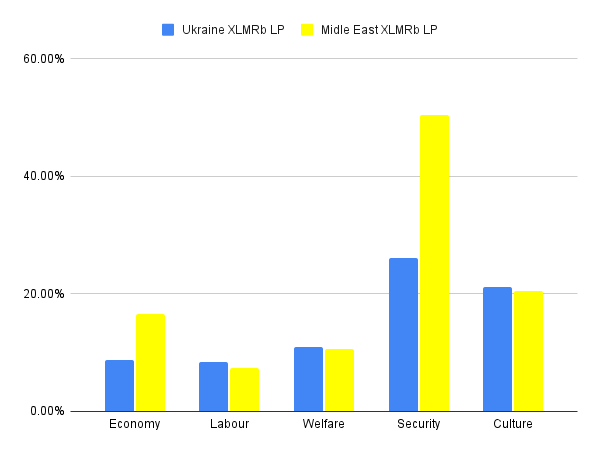
\includegraphics[width=0.5\textwidth]{figures/chart_sl_predictions_2.png}
  \caption{Preliminary research results comparing two EU migration crises using the Slovenian corpora predictions with a Zero-shot technique, showing the relative differences in Economy and Security news framing.}
  \label{fig:sl_predictions}
\end{figure}